%==============================================================

\chapter{Implementation}

The implementation consists of two separate parts. The first one contains the feature extraction and preparation of the data from the audio files. The result are stored in feature files. These features files then have to be processes with the Big Data framework Spark to compute the similarities between songs.\\ 
Both parts are implemented in Python and are able to be executed on computer clusters. The source code can be found in the appendices and can be pulled from github \cite{github-code}. Details for the usage of the python scripts are also documented there.

\section{Audio Feature Extraction}\label{simmet}

So far the required audio features have been selected in chapter \ref{audiofeat} as well as toolkits to extract those features from the audio data.
In chapter \ref{data} different sources for audio files have been presented. Chapter \ref{musly}, \ref{melsimc} and \ref{rhythmsimc} presented algorithms to pre-process the low-level features and use these to compute similarities. 
This chapter focuses on the selection of datasets to extract features from and the performance of the feature extraction and pre-processing software implementation.  

\subsection{Test Datasets}

Chapter \ref{datasets} introduced a range of MIR datasets but not all are fitting to the problems this thesis evaluates. To test the algorithms on the one hand a lot of data is needed, so the Free Music Archive with its over 100000 songs is a solid option for performance tests. However on the other hand the genre distribution in the FMA dataset is quite one sided. Most of the songs are tagged as experimental, electronic and rock. Also this dataset may not be really representative for actual popular music, a lot of the songs are live recordings with poor audio quality, possibly influencing the results.
The 1517 artists dataset offers 19 different genres with songs relatively equally distributed. For an objective evaluation of the proposed algorithms e.g. by genre recall this dataset is ideal. For cover song detection, the covers80 dataset is included as well.
The last source used in this thesis is the private music collection. This collection is biased towards metal music but due to the match with personal taste, it offers a subjective evaluation of the results of the similarity analysis. 
In conclusion that sums up to about 117000 songs for performance tests and about 12000 songs for a detailed evaluation of the algorithms in this thesis. As mentioned in \ref{datasets} all albums from the private music collections are cataloged as well and the associated document is in the appendices. For the first tests an even smaller sample dataset containing 10 songs out of 10 different genres was created from the private music collection and the list with the belonging songs is also in the appendices.

\begin{table}[h]
	\label{used_dsets}
	\begin{center}
		\begin{tabular}{|c||c|}
			\hline
			fma & 106.733 Songs\\
			\hline
			private & 8484 Songs\\
			\hline
			1517 artists & 3180 Songs\\
			\hline
			covers80 & 164 Songs (80 originals + 84 covers)\\
			\hline
		\end{tabular}
	\end{center}
	\caption{appropriate music datasets}
\end{table}
\FloatBarrier

\subsection{Feature Extraction Performance}

After evaluating the different features in the last three chapters, this section only discusses the performance of the feature extraction process without going too much into the details of the code for the feature post-processing. The post-processing of the features like the note estimation from the chroma features and the calculation of statistic features from the MFCCs was already explained in-depth in the previous chapters and is therefor left out here. The full code is in the appendices. 

\subsubsection{Librosa}

For most of the plots in the introduction section \ref{audiofeat} the python toolkit librosa was used because of its ease of use and very good documentation. The code example shows the necessary methods to extract the most important features like mfcc, chromagram and beats/ onsets.
\lstset{language=Python} 
\begin{pythonCode}[frame=single,label={lst:librosa},caption={librosa},captionpos=b]
path = ('music/guitar2.mp3')
x, fs = librosa.load(path)
mfcc = librosa.feature.mfcc(y=x, sr=fs, n_mfcc=12)
onset_env = librosa.onset.onset_strength(x, fs, aggregate=np.median)
tempo, beats = librosa.beat.beat_track(onset_envelope=onset_env,sr=fs)
times = librosa.frames_to_time(np.arange(len(onset_env)), sr=fs, hop_length= 512)
chroma = librosa.feature.chroma_stft(x, fs)
\end{pythonCode}	
But when extracting features from batches of audio data the librosa library turned out to be very slow. For a very small dataset of 100 songs, the extraction of just the mean, variance and covariance of the mfccs and the estimated notes from the chromagram took about 48 minutes. 
For larger datasets like the 1517 artists dataset the feature extraction process would have taken about 22 hours. 

\subsubsection{Essentia}

\cite{audiofeattoolb} compares different Audio feature extraction toolboxes and shows that essentia is a much faster alternative to librosa due to the underlying C++ Code and provides even more features, but it is a bit less well documented and requires more effort in implementation at the same time.\\ 
In the end the code to extract the necessary features had to be rewritten for the usage of essentia due to the slow performance of librosa. Essentia offers two different ways to handle audio files. The first one is to use the essentia standard library. It offers similar methods to librosa and uses an imperative programming style. The audio file has to be read, sliced and preprocessed by hand. 
The second way is to use essentia streaming. Basically a network of connected algorithms is created and they handle and schedule the "how and when" whenever a process is called.
The melodic and timbral features and the beat histograms are all computed with essentia. Only the rhythm patterns and rhythm histograms are computed in a separate step as stated below. 

\subsubsection{Essentia Standard}

In the final extractor code the mfcc calculation and beat histogram estimation is done with the essenia standard library, because it offers a fast and easy way to implement the basic feature extraction tasks. 
\begin{pythonCode}[frame=single,label={lst:esss},caption={essentia standard},captionpos=b]
audio = es.MonoLoader(filename=path, sampleRate=fs)()
hamming_window = es.Windowing(type='hamming')
spectrum = es.Spectrum()
mfcc = es.MFCC(numberCoefficients=13)
mfccs = numpy.array([mfcc(spectrum(hamming_window(frame)))[1] 
	for frame in es.FrameGenerator(audio, frameSize=2048, hopSize=1024)])
rhythm_extractor = es.RhythmExtractor2013(method="multifeature")
bpm, beats, beats_confidence, _, beats_intervals = rhythm_extractor(audio)
peak1_bpm, peak1_weight, peak1_spread, peak2_bpm, peak2_weight, peak2_spread, histogram =
	es.BpmHistogramDescriptors()(beats_intervals)
\end{pythonCode}

\subsubsection{Essentia Streaming}

The essentia streaming library is used to calculate the chroma features in the final code. It eases up the filtering with the high- and a lowpass filter. The audio signal is passed through various stages of processing and ultimately resulting in the chroma features of the high-pass filtered audio signal. 
%\newpage
\begin{pythonCode}[frame=single,label={lst:essst},caption={essentia streaming},captionpos=b]
loader = ess.MonoLoader(filename=path, sampleRate=44100)
HP = ess.HighPass(cutoffFrequency=128)
LP = ess.LowPass(cutoffFrequency=4096)
framecutter = ess.FrameCutter(frameSize=frameSize, hopSize=hopSize, 
	silentFrames='noise')
windowing = ess.Windowing(type='blackmanharris62')
spectrum = ess.Spectrum()
spectralpeaks = ess.SpectralPeaks(orderBy='magnitude', magnitudeThreshold=0.00001, 
	minFrequency=20, maxFrequency=3500, maxPeaks=60)
hpcp = ess.HPCP()
hpcp_key = ess.HPCP(size=36, referenceFrequency=440, bandPreset=False, minFrequency=20,
	maxFrequency=3500, weightType='cosine', nonLinear=False, windowSize=1.)
key = ess.Key(profileType='edma', numHarmonics=4, pcpSize=36, slope=0.6, 
	usePolyphony=True, useThreeChords=True)
pool = essentia.Pool()
loader.audio >> HP.signal
HP.signal >> LP.signal
LP.signal >> framecutter.signal    
framecutter.frame >> windowing.frame >> spectrum.frame
spectrum.spectrum >> spectralpeaks.spectrum
spectralpeaks.magnitudes >> hpcp.magnitudes
spectralpeaks.frequencies >> hpcp.frequencies
spectralpeaks.magnitudes >> hpcp_key.magnitudes
spectralpeaks.frequencies >> hpcp_key.frequencies
hpcp_key.hpcp >> key.pcp
hpcp.hpcp >> (pool, 'tonal.hpcp')
essentia.run(loader)
chroma = pool['tonal.hpcp'].T
\end{pythonCode}	

\subsubsection{Essentia performance}

The calculation with the essentia library for 100 songs took less than half of the time librosa needed. This is a significant improvement, however the essentia library uses only one CPU core so that performance was further improved by using the parallel python library as presented in the next code snippet.

\subsubsection{parallel python}

Multiple CPU cores get a part of the filelist of all songs and can compute the features fully parallel.
%\newpage
\begin{pythonCode}[frame=single,label={lst:pp},caption={parallel python},captionpos=b]
job_server = pp.Server()
job_server.set_ncpus(ncpus)
jobs = [ ]
for index in xrange(startjob, parts):
	starti = start+index*step
	endi = min(start+(index+1)*step, end)
	jobs.append(job_server.submit(parallel_python_process, (index, 
		filelist[starti:endi],1,1,1,1,1)))
	gc.collect()
times = sum([job() for job in jobs])
job_server.print_stats()
\end{pythonCode}
The computation time takes about 15.4 seconds per song and processor core. Using 4 CPU cores for 100 songs, the overall processing time could be reduced to about 385 seconds. 
\begin{equation} \label{eq:parallelp}
time = \frac{\#songs}{\#CPUs} \cdot 15.4s
\end{equation}
Parallel python also opens up the possibility to use a cluster instead of a single node PC.\\
For convenience, every processor gets a batch of files instead of single songs. For every batch different output files for the various features are created. The batch size determines the overall size of these feature-files. For example for the 1517 artists dataset a batch size of 400 songs was chosen, so overall 4 CPUs had to process 2 batches, resulting in 8 different output files with the chroma feature files being the largest with about 25MB per file.\\
One problem that appeared by using parallel python was that the memory usage was increasing over time. The explicit usage of the garbage collector and the deletion of unwanted objects also couldn't solve that problem. So after calculating a few hundred features the process ran out of memory and had to be restarted. By replacing parallel python with mpi4py this problem could be solved later. 

\subsubsection{rp\_extractor}

For the extraction of the rhythm patterns and rhythm histogram features as described in chapter \ref{rhythmsimc} the rp\_extractor tool provided by the TU Wien was used. Although running in parallel on all CPU cores on a single node, the extraction of the features from 100 songs takes about 442 seconds.

\subsubsection{performance on a single pc}

The extraction of the rhythm patterns and the rhythm histogram is performed by the rp\_extractor tool. The feature extraction and processing of all the other features (beat histogram, mfcc statistics, notes and beat-aligned chromagram) had to be implemented separately and different MIR toolkits were tested. 

\begin{figure}[htbp]
	\centering
	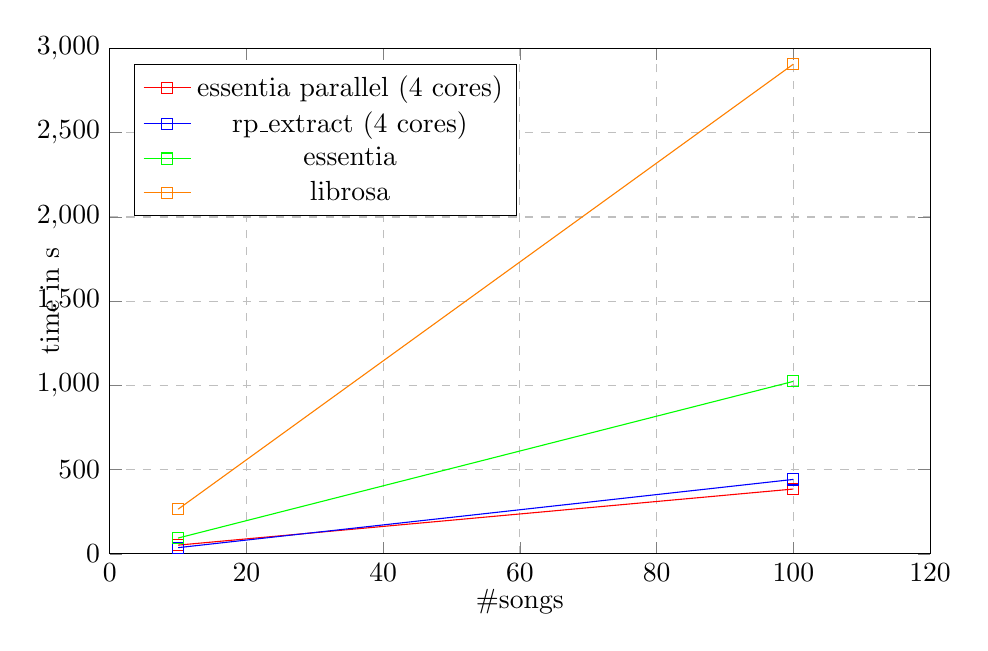
\begin{tikzpicture}
	\centering
	\begin{axis}[
	    %title={Performance of various toolkits},
		x label style={at={(axis description cs:0.5,-0.05)},anchor=north},
		y label style={at={(axis description cs:-0.05,.5)},rotate=0,anchor=south},
	    xlabel={\#songs},
	    ylabel={time in s},
	    xmin=0, xmax=120,
	    ymin=0, ymax=3000,
	    xtick={0,20,40,60,80,100,120},
	    ytick={0,500,1000,1500,2000,2500,3000},
	    legend pos=north west,
	    ymajorgrids=true,
	    grid style=dashed,
	    height=8cm,
	    width=12cm,
	    grid=major,
	]
	\addplot[
		color=red,
		mark=square,
		]
		coordinates {
		(10,52)(100,385)
		};
		\addlegendentry{essentia parallel (4 cores)}
	\addplot[
	    color=blue,
	    mark=square,
	    ]
	    coordinates {
	    (10,37)(100,442)
	    };
	    \addlegendentry{rp\_extract  (4 cores)}
	\addplot[
	    color=green,
	    mark=square,
	    ]
	    coordinates {
		(10,94)(100,1024)
	    };
	    \addlegendentry{essentia}
	\addplot[
	    color=orange,
	    mark=square,
	    ]
	    coordinates {
	    (10,265)(100,2907)
	    };
	    \addlegendentry{librosa}	    
	\end{axis}
	\end{tikzpicture}
	\caption{Performance of various toolkits on a single computer}
	\label{perfex}
\end{figure}
\noindent In summary the estimated time for the feature extraction on a single computer based on the performance measurements can be calculated and is listed below, leading to the conclusion that the extraction of the features for the full dataset including the FMA dataset can only be done with the help of a computing cluster.
\ \\
\textbf{Estimated feature extraction times}
\begin{itemize}
	\setlength\itemsep{-0.5em}
	\item 3h24 - 1517 artists - essentia parallel, single node, 4 CPU cores
	\item 3h54 - 1517 artists - rp\_extract
	\item 9h06 - private dataset - essentia parallel, single node, 4 CPU cores
	\item 10h24 - private dataset - rp\_extract
	\item (125h - full dataset - essentia parallel, single node, 4 CPU cores)
	\item (143h - full dataset - rp\_extract)
\end{itemize}

\subsubsection{performance on a cluster with mpi4py}

For the extraction of the features from the fma dataset on the computer cluster of the Friedrich-Schiller-University in Jena, the "ARA-cluster", parallel python had to be replaced with mpi4py. 
Mpi4py provides Python bindings for the Message Passing Interface standard (MPI) \cite{mpi4py}. 
Every compute process gets a rank number and is aware of the overall count of all processes. With these two values the file list of all audio files is split and each process only processes the according files. The audio files were stored in a parallel cluster file system called beegfs \cite{beegfs}. Equally to the implementation using parallel python every process stores the results in separate output files, each of them containing batches of 25 songs.\\
All audio files larger than 25MB were filtered out of the fma dataset to avoid memory overflows, still leaving 102813 songs out of the 106733 songs to process. A total of 36 compute nodes were used. Every node had 192GB of RAM and 36 CPU cores (72 using hyper-threading (HT)). To increase the available Memory per CPU, only 18 CPU cores per node were used. Overall 648 processses were spawned. During the computation of the audio features with essentia one out of the 648 processes ran out of memory, so only 102793 out of the 102813 songs were processed. For performance tests this doesn't make a large difference but for future work, the feature extraction script should be adapted accordingly. 
The extraction of the features took 1439s (fastest process) to 1950s (slowest). With a better balancing and messaging between the processes, the task could be distributed in a way where idle tasks take parts of the file list from tasks that are still processing. 

\begin{pythonCode}[frame=single,label={lst:mpi4py},caption={mpi4py},captionpos=b]
comm = MPI.COMM_WORLD   # get MPI communicator object
size = comm.size        # total number of processes
rank = comm.rank        # rank of this process
status = MPI.Status()   # get MPI status object
files_per_part = 25
start = 0
last = len(filelist)
parts = (len(filelist) / files_per_part) + 1
step = (last - start) / parts + 1
for index in xrange(start + rank, last, size):
    if index < parts:        
        starti = start+index*step
        endi = min(start+(index+1)*step, last)
        parallel_python_process(index, filelist[starti:endi])
\end{pythonCode}

\noindent For the extraction of the rhythm features with the rp\_extract tool, the script of the TU Wien was adapted for usage with mpi4py as well. The same amount of processes is spawned on the cluster (648), but each of the processes is able to make use of 2 CPU cores plus HT. The fastest process finished after 1657s and the slowest one took 1803s.

\subsubsection{Total amount of songs}

Due to the above mentioned filtering of audio files larger than 25MB and due to the fact that the rhythm pattern extraction script is not able to handle some audio file formats like Ogg Vorbis, not all features from all songs could be extracted. So in the end the overall count of songs where features could be extracted is 114310.\\


